\documentclass[../doc.tex]{subfiles}

\begin{document}
\section{Réalisation de l'intelligence artificielle}
Plus spécifique aux mécaniques de l'intelligence artificielle et des NPC,
 trois types de personnages doivent être implémentés à la carte:
\begin{itemize}
    \item Des NPC qui restent bloqués sur place et qui discutent en groupe
    \item Des IA qui se déplacent de manière aléatoire (ou qui patrouillent)
    \item Des NPC qui effectuent des animations précises
        (juste pour le décor plus réaliste et travaillé)
\end{itemize}

Pour créer l'IA, nous utiliserons le système de Nav Mesh intégré à Unity, zone où les NPC peuvent naviguer pour aller d'un point A vers un point B.
On appelle cela du pathfinding; c'est-à-dire que l'IA va calculer le meilleur chemin possible pour atteindre une position.
Nous avons déjà réalisé un début d'IA qui selon une liste de positions, se déplace d'un point à un autre avant de revenir à sa position initiale.

\begin{figure}[!htb]
    \centering
    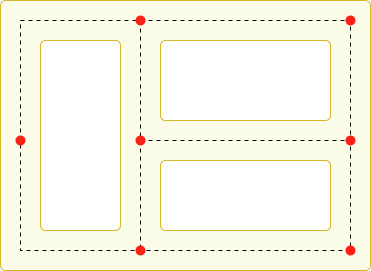
\includegraphics[scale=0.5]{NavPatrolMaze.jpg}
    \caption{Schéma d'un mouvement de patrouille}
\end{figure}

\end{document}